\section{Siamese gems}
\label{sec:siamese-gems}

\subsection{Forced vertices}

The \emph{sides} of the grid are its first and last rows and columns.

\begin{lemma}[Forced vertices]
\label{lem:forced}
Let $S$ be an arrangement of order $n\ge2$. The following points are vertices of $\mathcal G(S)$: the points over the four corner cells; the points carrying the entries $1$ and $N$; and, for each side, the points over the cells of the smallest and of the largest entry on that side.
\end{lemma}

\begin{proof}
A point that is the unique maximiser of a linear functional over the $N$ points is a vertex.
The entries are distinct, so $\mp z$ have unique maximisers where $s=1$ and $s=N$.
The functional $-x+y$ attains its maximum only at the top-left corner, and similarly for the other corners.
On the left column $x=-\frac{n-1}2$, while $x\ge-\frac{n-1}2+1$ elsewhere; for $\varepsilon=1/N$ the functional $-x+\varepsilon z$ exceeds $\frac{n-1}2-\frac12$ on the left column and is at most $\frac{n-1}2-\frac12$ elsewhere, so its unique maximiser is the point of largest height on the left column; $-x-\varepsilon z$ gives the smallest, and the other sides follow by symmetry.
\end{proof}

In the language of \Cref{prop:subdivisions}, the lemma says that the vertices of $\operatorname{conv}A$ and the extreme heights over each edge of $\operatorname{conv}A$ are used by every pair of subdivisions $\mathcal S(z),\mathcal S(-z)$.
For order four the forced vertices number between $4$ and $13$ and in general other points are vertices as well (\Cref{sec:census}).
For the Siamese squares nothing else is.

\subsection{The theorem}

The \emph{Siamese} (de la Loub\`ere) square of odd order $n=2m+1$ \cite{loubere1693} has $1$ in the middle cell of the top row; each next entry is placed one step up and one step to the right, cyclically, or one step down if that cell is occupied.
For $n=5$ it is
\[
\begin{pmatrix}17&24&1&8&15\\23&5&7&14&16\\4&6&13&20&22\\10&12&19&21&3\\11&18&25&2&9\end{pmatrix},
\]
and for $n=3$ it is a $D_4$-image of the Lo Shu.
Write $\langle t\rangle\in\{0,\dots,n-1\}$ for the residue of $t$ modulo $n$.

\begin{theorem}[Siamese gems]
\label{thm:siamese}
Let $S$ be the Siamese square of odd order $n=2m+1\ge3$. The vertices of $\mathcal G(S)$ are exactly the forced vertices of \Cref{lem:forced}: the eight boundary points for $n=3$, and for $n\ge5$ the twelve points over the cells
\[
\begin{array}{lll}
(0,0)\colon \bar s+m+2, & (0,m-1)\colon N-1, & (0,m)\colon 1, \\
(0,2m)\colon \bar s+m, & (m-1,0)\colon N-m, & (m,0)\colon m+2, \\
(m,2m)\colon N-m-1, & (m+1,2m)\colon m+1, & (2m,0)\colon \bar s-m, \\
(2m,m)\colon N, & (2m,m+1)\colon 2, & (2m,2m)\colon \bar s-m-2,
\end{array}
\]
listed with their entries. For $n\ge5$ the gem has $f$-vector $(12,26,16)$, with $12$ triangular and $4$ quadrilateral facets, and $\operatorname{Iso}(\mathcal G(S))=\operatorname{Iso}(P_S)=\{\mathrm{id},-\mathrm{id}\}$.
\end{theorem}

So the vertex fraction $12/n^2$ tends to zero, and the combinatorial type of the gem does not depend on $n\ge5$.

\begin{proof}
\emph{Step 1: closed form.}
We show $s(i,j)=n\langle i+j-m\rangle+\langle i+2j-2m\rangle+1$, the classical description of the Siamese square as a linear square \cite{andrews1960magic}.
The map $\kappa(i,j)=(\langle i+j-m\rangle,\langle i+2j-2m\rangle)$ is a bijection of $\Z_n^2$ (determinant $1$), and $\kappa(0,m)=(0,0)$.
Write $k-1=nq+r$ with $0\le r<n$; we prove by induction on $k$ that the entry $k$ is placed in the cell $\kappa^{-1}(q,r)$.
This holds for $k=1$. Suppose it holds for $1,\dots,k$, with $k$ in the cell $c=\kappa^{-1}(q,r)$; the occupied cells are $\kappa^{-1}(q',r')$ with $nq'+r'<k$.
The up-right move $(i,j)\to(i-1,j+1)$ keeps $i+j$ and increases $i+2j$ by $1$, so it leads to $\kappa^{-1}(q,\langle r+1\rangle)$.
If $r<n-1$, this cell is empty and is the cell prescribed for $k+1$.
If $r=n-1$, i.e.\ $n\mid k$, it is the cell $\kappa^{-1}(q,0)$ of the entry $nq+1$, so the move is blocked; the downward move $(i,j)\to(i+1,j)$ increases both $i+j$ and $i+2j$ by $1$ and leads to the empty cell $\kappa^{-1}(q+1,0)$, the cell prescribed for $k+1=n(q+1)+1$.
(Thus each run of $n$ entries fills one broken diagonal $i+j\equiv\text{const}$.)

\emph{Step 2: the forced vertices.}
In every row and every column the leading digit $\langle i+j-m\rangle$ takes each value in $\{0,\dots,n-1\}$ once, so the largest entry of a side is in the cell where this digit is $n-1$ and the smallest where it is $0$.
On the top row $i=0$ this gives $j=m-1$ with entry $n(n-1)+\langle-2\rangle+1=N-1$, and $j=m$ with entry $1$; on the bottom row $i=2m$, $j=m$ with entry $n(n-1)+n=N$, and $j=m+1$ with entry $\langle n+1\rangle+1=2$; on the left column $j=0$, $i=m-1$ with entry $n(n-1)+\langle-m-1\rangle+1=N-m$, and $i=m$ with $\langle-m\rangle+1=m+2$; on the right column $j=2m$, $i=m$ with entry $n(n-1)+\langle3m\rangle+1=N-m-1$, and $i=m+1$ with $\langle3m+1\rangle+1=m+1$.
The corner entries follow in the same way.
The entries $1$ and $N$ are among the side extremes, and for $m\ge2$ the eight side cells are distinct and are not corners; so the forced vertices are the twelve listed points. For $m=1$ the side extremes are the corners and the midpoints of the sides.
It remains to show that no other point is a vertex.
For $n=3$ this holds since the only other point is the centre $\mathbf 0$, an interior point; let $m\ge2$.

\emph{Step 3: affine reduction to five layers.}
With $x=j-m$, $y=m-i$ and $\langle t\rangle=t-n\lfloor t/n\rfloor$ the closed form gives
\begin{gather*}
z=\lambda(x,y)+n\,\zeta(x,y),\qquad \lambda(x,y)=n(x-y+m)+(2x-y+m)+1-\bar s,\\
\zeta(x,y)=-n\Big\lfloor\tfrac{x-y+m}{n}\Big\rfloor-\Big\lfloor\tfrac{2x-y+m}{n}\Big\rfloor .
\end{gather*}
The map $\Phi(x,y,z)=(x,y,(z-\lambda(x,y))/n)$ is an affine bijection that preserves vertical lines, so $\Phi(\mathcal G(S))=\operatorname{conv}\{(x,y,\zeta(x,y))\}$ has the same face lattice and vertex cells as $\mathcal G(S)$; equivalently, $\mathcal S(\pm z)=\mathcal S(\pm\zeta)$.
For $|x|,|y|\le m$ both floors lie in $\{-1,0,1\}$, and a case check of the two floors shows that $\zeta$ takes five values, on the lattice points of five convex lattice polygons in the box $|x|,|y|\le m$ (\Cref{fig:siamese-layers}a):
$\zeta=n+1$ on $\Lambda_{+2}=\{y\ge x+m+1\}=\operatorname{conv}\{(-m,m),(-1,m),(-m,1)\}$;
$\zeta=1$ on $\Lambda_{+1}=\{2x+m+1\le y\le x+m\}=\operatorname{conv}\{(-m,0),(-m,1-m),(-1,m-1)\}$;
$\zeta=0$ on $\Lambda_{0}=\{|y-2x|\le m\}=\operatorname{conv}\{(-m,-m),(0,m),(m,m),(0,-m)\}$;
and $\zeta=-1$, $-(n+1)$ on $\Lambda_{-1}=-\Lambda_{+1}$, $\Lambda_{-2}=-\Lambda_{+2}$.

\emph{Step 4: the hull.}
Let $v_1,\dots,v_{12}$ be the images under $\Phi$ of the twelve forced vertices and $u_1,\dots,u_4$ the remaining four vertices of the layer polygons; their coordinates are in \Cref{tab:slacks}.
Let $Q$ be the polyhedron defined by the inequalities
\begin{align*}
&(1)\ \zeta\le 2m+2, \qquad (2)\ y\le m, \qquad (3)\ -x\le m, \qquad (8)\ -2y+\zeta\le 2m,\\
&(4)\ -2(m{+}1)x+(2m{+}1)y-m\zeta\le m(2m{+}1),\qquad (7)\ 2mx-y+m\zeta\le m(2m{-}1),\\
&(5)\ 2(m{+}1)x-2(m{+}1)y+(2m{+}1)\zeta\le 2m(m{+}1),\\
&(6)\ 2m(m{+}2)x-(2m^2{+}2m{-}1)y+m(2m{+}1)\zeta\le m(2m^2{+}2m{-}1),
\end{align*}
and their images $(1')$--$(8')$ under $\mathbf q\mapsto-\mathbf q$.
\Cref{tab:slacks} lists the slack (right-hand side minus left-hand side) of $(1)$--$(8)$ at the sixteen layer vertices.
Every entry is $0$ or a product of factors that are positive for $m\ge2$, and the set of layer vertices is centrally symmetric, so all sixteen inequalities hold at all layer vertices and hence, by convexity, at all points $(x,y,\zeta)$: $\Phi(\mathcal G(S))\subseteq Q$.
The zeros of the table show that the planes $(1)$--$(8)$ contain the following $v_k$, in cyclic order:
\[
\begin{array}{llll}
(1)\colon v_1v_2v_3, & (2)\colon v_1v_2v_8v_7, & (3)\colon v_1v_3v_5v_4, & (4)\colon v_1v_4v_7,\\
(5)\colon v_2v_3v_6, & (6)\colon v_2v_6v_9, & (7)\colon v_2v_8v_9, & (8)\colon v_3v_5v_6,
\end{array}
\]
with the antipodal lists for $(1')$--$(8')$ ($v_{10}=-v_1$, $v_{11}=-v_3$, $v_{12}=-v_2$, $v_9=-v_4$, $v_8=-v_5$, $v_7=-v_6$).
Hence each of the sixteen planes meets $P=\operatorname{conv}\{v_1,\dots,v_{12}\}\subseteq Q$ in a polygon, which is therefore a facet of $P$.
These sixteen polygons ($12$ triangles and the $4$ quadrilaterals $(2),(3),(2'),(3')$, which are convex in the cyclic orders given) have $26$ edges, each shared by exactly two of them; since the facet-adjacency graph of a $3$-polytope is connected, they are all the facets of $P$, and $P=Q$.
As $P\subseteq\Phi(\mathcal G(S))\subseteq Q=P$, the gem is the image of $P$ under $\Phi^{-1}$, with vertex set the twelve forced vertices and $f$-vector $(12,26,16)$.

\emph{Step 5: isometries.}
$S$ is associative (by the closed form, $s(i,j)+s(2m-i,2m-j)=N+1$), so $\operatorname{Iso}(P_S)=\{\pm\mathrm{id}\}$ by \Cref{thm:pointset}.
An isometry of $\mathcal G(S)$ fixes the centroid $\mathbf 0$ of its centrally symmetric vertex set and is orthogonal.
In the original coordinates
$v_1=(-m,m,m+2)$, $v_2=(-1,m,2m^2+2m-1)$, $v_3=(-m,1,2m^2+m)$, $v_4=(-m,0,-2m^2-m+1)$, $v_5=(-m,-m,-m)$, $v_6=(0,-m,2m^2+2m)$, and the other six are their negatives.
The squared norms
$3m^2<3m^2+4m+4<4m^4+4m^3-2m^2-2m+1<4m^4+4m^3+2m^2+1<4m^4+8m^3+m^2-4m+2<4m^4+8m^3+5m^2$
of $v_5,v_1,v_4,v_3,v_2,v_6$ are distinct for $m\ge2$, so an isometry maps each $v_k$ to $\pm v_k$.
The inner products of $v_1$ with $v_2,\dots,v_6$ are $2m^3+7m^2+4m-2$, $m(2m^2+6m+3)$, $-(2m^3+4m^2+m-2)$, $-m(m+2)$, $m(2m^2+5m+4)$, all non-zero, so all signs agree with that of $v_1$, and the isometry is $\pm\mathrm{id}$.
\end{proof}

\begin{table}[htbp]
\centering
\caption{Proof of \Cref{thm:siamese}, Step 4: the sixteen vertices of the layer polygons $\Lambda_{+2},\Lambda_{+1},\Lambda_0,\Lambda_{-1},\Lambda_{-2}$ (groups of rows) and the slacks of the inequalities $(1)$--$(8)$ at them, as polynomials in $m$; zeros in bold. All non-zero entries are positive for $m\ge2$. The points $v_1,\dots,v_{12}$ are the images of the forced vertices, $u_1,\dots,u_4$ are not vertices of the gem.}
\label{tab:slacks}
\scriptsize
\setlength{\tabcolsep}{4pt}
\resizebox{\textwidth}{!}{\begin{tabular}{l l cccccccc}
\toprule
point & $(x,y,\zeta)$ & (1) & (2) & (3) & (4) & (5) & (6) & (7) & (8)\\
\midrule
$q_{1}$ & $(-m,m,2m+2)$ & $\mathbf{0}$ & $\mathbf{0}$ & $\mathbf{0}$ & $\mathbf{0}$ & $2(m-1)(m+1)$ & $2m(m-1)(m+2)$ & $2m(m-1)$ & $2(m-1)$\\
$q_{2}$ & $(-1,m,2m+2)$ & $\mathbf{0}$ & $\mathbf{0}$ & $m-1$ & $2(m-1)(m+1)$ & $\mathbf{0}$ & $\mathbf{0}$ & $\mathbf{0}$ & $2(m-1)$\\
$q_{3}$ & $(-m,1,2m+2)$ & $\mathbf{0}$ & $m-1$ & $\mathbf{0}$ & $(m-1)(2m+1)$ & $\mathbf{0}$ & $(m-1)(2m+1)$ & $(m-1)(2m-1)$ & $\mathbf{0}$\\
\addlinespace[2pt]
$q_{4}$ & $(-m,0,1)$ & $2m+1$ & $m$ & $\mathbf{0}$ & $\mathbf{0}$ & $4m^{2}+2m-1$ & $2m(2m^{2}+2m-1)$ & $2m(2m-1)$ & $2m-1$\\
$q_{13}$ & $(-m,1-m,1)$ & $2m+1$ & $2m-1$ & $\mathbf{0}$ & $(m-1)(2m+1)$ & $2m^{2}+2m+1$ & $(m+1)(2m^{2}+2m-1)$ & $4m^{2}-3m+1$ & $1$\\
$q_{14}$ & $(-1,m-1,1)$ & $2m+1$ & $1$ & $m-1$ & $m-1$ & $4m^{2}+2m-1$ & $(m+1)(4m^{2}-2m+1)$ & $(m+1)(2m-1)$ & $4m-3$\\
\addlinespace[2pt]
$q_{5}$ & $(-m,-m,0)$ & $2(m+1)$ & $2m$ & $\mathbf{0}$ & $2m^{2}$ & $2m(m+1)$ & $2m^{2}(m+2)$ & $2m(2m-1)$ & $\mathbf{0}$\\
$q_{6}$ & $(0,-m,0)$ & $2(m+1)$ & $2m$ & $m$ & $2m(2m+1)$ & $\mathbf{0}$ & $\mathbf{0}$ & $2m(m-1)$ & $\mathbf{0}$\\
$q_{7}$ & $(0,m,0)$ & $2(m+1)$ & $\mathbf{0}$ & $m$ & $\mathbf{0}$ & $4m(m+1)$ & $2m(2m^{2}+2m-1)$ & $2m^{2}$ & $4m$\\
$q_{8}$ & $(m,m,0)$ & $2(m+1)$ & $\mathbf{0}$ & $2m$ & $2m(m+1)$ & $2m(m+1)$ & $2m(m-1)(m+1)$ & $\mathbf{0}$ & $4m$\\
\addlinespace[2pt]
$q_{9}$ & $(m,0,-1)$ & $2m+3$ & $m$ & $2m$ & $2m(2m+1)$ & $2m+1$ & $\mathbf{0}$ & $\mathbf{0}$ & $2m+1$\\
$q_{15}$ & $(m,m-1,-1)$ & $2m+3$ & $1$ & $2m$ & $(m+1)(2m+1)$ & $2m^{2}+2m-1$ & $(m-1)(2m^{2}+2m-1)$ & $m-1$ & $4m-1$\\
$q_{16}$ & $(1,1-m,-1)$ & $2m+3$ & $2m-1$ & $m+1$ & $4m^{2}+m+1$ & $2m+1$ & $(m-1)(2m+1)$ & $(m-1)(2m-1)$ & $3$\\
\addlinespace[2pt]
$q_{10}$ & $(m,-m,-2m-2)$ & $4(m+1)$ & $2m$ & $2m$ & $2m(2m+1)$ & $2(m+1)^{2}$ & $2m(m^{2}+m+1)$ & $2m^{2}$ & $2(m+1)$\\
$q_{11}$ & $(m,-1,-2m-2)$ & $4(m+1)$ & $m+1$ & $2m$ & $(m+1)(2m+1)$ & $4m(m+1)$ & $(m+1)(4m^{2}-2m+1)$ & $(m+1)(2m-1)$ & $4m$\\
$q_{12}$ & $(1,-m,-2m-2)$ & $4(m+1)$ & $2m$ & $m+1$ & $2(m^{2}+m+1)$ & $4m(m+1)$ & $2m(2m^{2}+2m-1)$ & $2m(2m-1)$ & $2(m+1)$\\
\bottomrule
\end{tabular}
}
\end{table}

All entries of \Cref{tab:slacks} and the closure of the facet list are verified by \texttt{anc/siamese\_slacks.py} in exact polynomial arithmetic, and the theorem is checked against exact hull computations for $n=3,5,\dots,41$ (\texttt{anc/verify\_revision.py}).
For $m=1$ several entries vanish and the four triangles degenerate.

\begin{figure}[htbp]
\centering
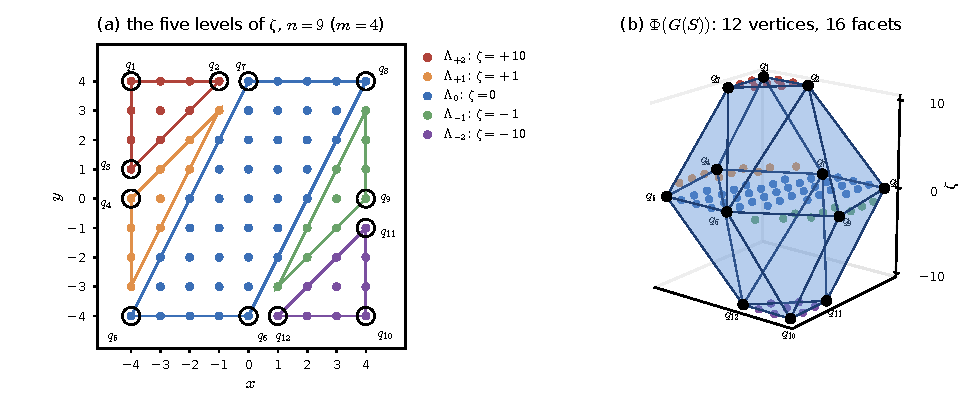
\includegraphics[width=0.88\textwidth]{figures/fig_siamese_layers.pdf}
\caption{The Siamese gem of order $n=9$ after the affine reduction $\Phi$. (a)~The $81$ cells coloured by the layer value $\zeta\in\{\pm10,\pm1,0\}$, with the five layer polygons outlined and the twelve vertex cells $v_1,\dots,v_{12}$ circled. (b)~$\Phi(\mathcal G(S))$ with its $12$ vertices and $16$ facets. The combinatorics of the layer polygons does not depend on $m\ge2$.}
\label{fig:siamese-layers}
\end{figure}

\begin{remark}[Linear squares]
\label{rem:linear}
The Siamese square is a \emph{linear} (cyclic) square $s(c)=n\langle\mathbf u\cdot c+\alpha\rangle+\langle\mathbf w\cdot c+\beta\rangle+1$ with $\mathbf u,\mathbf w\in\Z_n^2$ and $\alpha,\beta\in\Z_n$, and for fixed integer vectors $\mathbf u,\mathbf w$ the same shear reduces the lift to a number of layers that does not depend on $n$.
The gems of linear squares do not share the bounded vertex count, however.
Over all linear magic squares of order $n$ (\texttt{anc/linear\_squares.py}, exact hulls) the vertex counts range over $[11,18]$ for $n=5$ ($184$ $D_4$-classes), $[12,25]$ for $n=7$ ($3159$ classes), $[12,31]$ for $n=9$ ($441$ classes) and $[12,36]$ for $n=11$ ($89{,}125$ classes); the minimum $12$ is attained by exactly two classes for $n=7,9,11$, one of them the Siamese square. For $n=7$ the other is the square $n\langle i+2j-2m\rangle+\langle i+j-m\rangle+1$ obtained by exchanging the two digits of the closed form; it is magic for every odd $n$, and its gem has $f$-vector $(12,24,14)$ for $n=5,7,\dots,31$.
\end{remark}
